% !TEX TS-program = pdflatex
% !TEX encoding = UTF-8 Unicode

% This is a simple template for a LaTeX document using the "article" class.
% See "book", "report", "letter" for other types of document.

\documentclass[11pt]{article} % use larger type; default would be 10pt

%\usepackage[utf8]{inputenc} % set input encoding (not needed with XeLaTeX)

%%% Examples of Article customizations
% These packages are optional, depending whether you want the features they provide.
% See the LaTeX Companion or other references for full information.

%%% PAGE DIMENSIONS
\usepackage{geometry} % to change the page dimensions
\geometry{letterpaper} % or letterpaper (US) or a5paper or....
% \geometry{margin=2in} % for example, change the margins to 2 inches all round
% \geometry{landscape} % set up the page for landscape
%   read geometry.pdf for detailed page layout information

\usepackage{graphicx} % support the \includefigureics command and options

% \usepackage[parfill]{parskip} % Activate to begin parafigures with an empty line rather than an indent

%%% PACKAGES
\usepackage{booktabs} % for much better looking tables
\usepackage{array} % for better arrays (eg matrices) in maths
\usepackage{paralist} % very flexible & customisable lists (eg. enumerate/itemize, etc.)
\usepackage{verbatim} % adds environment for commenting out blocks of text & for better verbatim
\usepackage{subfig} % make it possible to include more than one captioned figure/table in a single float
% These packages are all incorporated in the memoir class to one degree or another...
\usepackage{hyperref}
\usepackage{pdfpages}
%%% HEADERS & FOOTERS
\usepackage{fancyhdr} % This should be set AFTER setting up the page geometry
\pagestyle{fancy} % options: empty , plain , fancy
\renewcommand{\headrulewidth}{0pt} % customise the layout...
\lhead{}\chead{}\rhead{}
\lfoot{}\cfoot{\thepage}\rfoot{}

%%% SECTION TITLE APPEARANCE
\usepackage{sectsty}
\allsectionsfont{\sffamily\mdseries\upshape} % (See the fntguide.pdf for font help)
% (This matches ConTeXt defaults)

%%% ToC (table of contents) APPEARANCE
\usepackage[nottoc,notlof,notlot]{tocbibind} % Put the bibliofigurey in the ToC
\usepackage[titles,subfigure]{tocloft} % Alter the style of the Table of Contents
\renewcommand{\cftsecfont}{\rmfamily\mdseries\upshape}
\renewcommand{\cftsecpagefont}{\rmfamily\mdseries\upshape} % No bold!

%%% END Article customizations

%%% The "real" document content comes below...

\title{Cluster Analsysis of SS data from 2005 to 2012}
\author{Tim Pobst}
\date{Dec. 2013} % Activate to display a given date or no date (if empty),
         % otherwise the current date is printed 

\begin{document}
\maketitle

\section{Infuential Observations}

Cluster analysis performed by Tim Pobst and David Mercer.  David Mercer is a student employee of OIT, he helps with statistics.
    
The excel file used is called Complete 387 stream chemistry 1993 to 2012.  The data sheet used is labeled dataset.  Furthermore in order to identify trends only the years 2005 to 2012 were used.  This is because the frequency of sampling needs to be constant in order to detect trends, which is used in finding outliers.  The years of 2005 to 2012 mark the period for the current stream survey network and is also the largest data set with a constant frequency.  It contains the six watersheds I was asked to evaluate plus Hazel creek watershed.

Ward’s minimum variance method is affected by outliers.  The first data analysis performed was to find the outliers in the data.  Figures were created of pH vs. Month, Elevation class, Elevation (m).  These are shown in figures 1 through 3.  \hyperref[CAGraph1]{Figure 1} is pH vs. Month; this was figured to look for seasonality and closely resembles the figure of pH vs. Time.  As can be seen in figure 1, there are many outliers, which are the data points above and below the boxplots.  An outlier is more than two quartile lengths away from the mean.  \hyperref[CAGraph2]{Figure 2} is pH vs. Elevation class which was graphed in order to see a trend in pH and elevation.  In this figure class 3 and 9 have very large pH ranges which occur in just 500 ft. of elevation.  The reasons for these large ranges will be shown in pH vs. watershed and site ID.  Also in figure 2 there are many low outliers for elevation classes 5 and 6.  \hyperref[CAGraph3]{Figure 3} was created in order to see what was making elevation classes 3 and 9 so large.  The high pH values in elevation class 3 and to some extent 4 can be accounted for as part of Abrams watershed.  Abrams watershed is underlain by cades sandstone and has high natural ANC to buffer any added acids.  The whole Abrams watershed will be taken out as an outlier.  There many low data points in the range of elevation class 9.  These points are well grouped and are sites with consistently low pH values.  They turn out to be sites 252 and 237 which are affected by road cuts into an Anakeesta formation which is high in sulfur and  lowers the pH drastically.  These sites have means that are so low that they will be taken out as to influential.    Also noticeable are many low outliers, many of these can be attributed to storm flow.  Storm flow periodically lowers pH as storms increase Nitrates and Sulfates in the stream.  Storm flow is a column in the data and is characterized as the top 5$\%$ of stream flows.  Storm flow is also removed as an outlier.\hyperref[CAGraph6]{Figure 4} shows pH vs. Site ID without any of the previously stated influential observations.  Many of the lower outliers can be explained by storm flow conditions.  Figure 4 is the final figure concerning outliers.  Abrams watershed, storm flow, and sites 237 and 252 have all been taken out.  There are three sites left with low means.  Sites 4 and 137 are both from Cosby and Cosby only has 4 sites.  All three of the means of these sites are within the outer quartiles of other sites; therefore they are not outliers in themselves.
    
\begin{table}[htbp]
\caption{Used for detection of influential observations}
\begin{tabular}{lllllll}
\toprule
\multicolumn{7}{l}{Summary Section of pH (Including Abrams)}  \\ 
\midrule
Count & Mean & Standard Deviation & Standard Error & Minimum & Maximum & Range \\ 
1397 & 6.485132 &0.6049951 & 0.01618653 &4.215162 & 8.099278 & 3.8841 \\ 
\midrule
\multicolumn{7}{l}{Summary Section of pH (Excluding Abrams)} \\ 
\midrule
Count & Mean & Standard Deviation & Standard Error & Minimum & Maximum & Range \\ 
1239 & 6.403315 & 0.5529732 & 0.01570972 & 4.215162 & 7.370326 & 3.1552 \\ 
\midrule
\multicolumn{7}{l}{Summary Section of pH (Excluding Abrams and storm flow and sites 237 and 252)}\\ 
\midrule
Count & Mean & Standard Deviation & Standard Error & Minimum & Maximum & Range \\ 
614 & 6.511126 & 0.3904229 & 0.01575619 & 4.659964 &7.370326 & 2.7104 \\ 
\bottomrule
\end{tabular}
\label{Data Summary}
\end{table}


Here we have some summary statistics taken while removing the outliers.  The drop in count is due mainly to storm flow.  The mean does not change drastically from all outliers being present to removing all outliers.  The standard deviation does drop two tenths from everything included to all outliers taken out.  Of course, the max is dropped when Abrams is taken out, and the minimum is raised when storm flow and sites 237 and 252 are removed, shrinking the range by a full pH point.  These are all signs that we are successfully removing outliers. 
    
The next couple of figures (figures 5 through 7) are the similar to the earlier figures except they do not have any outliers.  The most important figure is \hyperref[CAGraph8]{Figure 5} because it is pH vs. Elevation class.  If we want to run a cluster analysis to get new elevation classes by pH then we hope to see this figure show a clear, well defined trend.  But we don't ,elevation class 3 and 10 have much lower means than the rest of the elevation classes.  Class 3 contains Cosby watershed which may account for its being so low, specifically site $\#$4.  Class 10 is low because of site $\#$234 from Road prong.  And then there are a couple of low outliers in the upper elevation classes.  If the outliers could not be explained then they were not excluded.

\section{methods}
Ward’s minimum variance is a distance method by which clusters are created in order that the total variance of the data is minimized.  It begins with every data point as its own cluster and then combines the two clusters that will create the least amount of change in the total variance.  This is done until there is only one cluster left.  At this point, the dendrogram is evaluated to choose how many clusters are best.  This is usually done by looking at the distance, or in Ward’s case amount of variation added, between the clusters.  Large jumps in distance usually indicate natural clusters.

The goal for this cluster analysis is to create elevation bands.  A correlation matrix was created in JMP in order to see which variables correlated well enough with elevation to create clusters.  The variables chosen were pH, ANC, Nitrate, and Sulfate.   The first analysis identified two more site outliers; these sites were generally placed into clusters all on their own.  Sites $\#251$ in Oconaluftee is put into a cluster almost by itself at all numbers of clusters.  This could mean that it is an outlier.  After this site was removed site, $\#253$ would be placed in a cluster all on its own.  Both of these sites are affected by anakeesta rock formations, and are near site $\#252$ was taken out early as an outlier.

After these, no more obvious outliers were found.  A five cluster and a fifteen cluster grouping was chosen because they looked most natural.  You can see this in the dendrogram by the long lines formed before a cluster is joined, and they are the largest jumps in the clustering history.

\section{Results}%results have changed slightly, from looking at the dendrogram the choices for clusters are 15 or 5, distributions of siteID, Stream System, elevation belonging to clusters.  try clusters belonging to these groups  How to make distributions in JMP
Copies of  {\it 5clusters.pdf} and {\it 15clusters.pdf} must be in the folder lables {\it figures} for these links to work.\\
\\
\href{run:figures/5clusters.pdf}{5 Cluster Distributions}\\
\\ 
\href{run:figures/15clusters.pdf}{15 Cluster Distributions}\\

The results are summarized with distribution analysis from JMP.  They are the distribution of pH, Stream System, and elevation within each proposed cluster.  The first distribution is the pH distribution, it is the closest to normal.  Another useful distribution which I did not show here is which sites belong to which clusters. These do not help much with elevation and pH but it may help determine why certain clusters formed.

\subsection{5 Clusters}
Cluster 1 is $68\%$ West Prong Little Pidgeon which is known as the Road stream system.  It contains 95 observations and the elevation ranges from 800 to 1700 meters.  This is the smallest cluster and the one with the largest elevation range.

Cluster 2 is dominated by the Cosby stream system at 53$\%$ while including all of the other stream systems.   Because it is dominated by Cosby which has only four sites that are fairly close together, the elevation is very tightly packed compared to the other clusters.

Cluster 3 is mostly West Prong Little Pidgeon and Cataloochee.  It contains 215 observations and ranges from 1000 meters to 1600 meters in elevation.  It contains the largest outliers of all the clusters.

Cluster 4 contains all road stream system sites.  It has 149 observations and the elevations are split around 360 meters and 440 meters.

Cluster 5 is $59\%$ Cataloochee.  It has 307 observations but despite being the largest cluster its elevation ranges only 300 meters.

\subsection{15 Clusters}
The output for the 15 cluster distributions from JMP gave me a lot of trouble.  Some of the outputs are cut off at the top which includes the titles but I assure you all of the distributions are in order.

I included the 15 cluster grouping just for some variety, but the way that hierarchical clustering works the 15 clusters will be just like the 5 clusters but divided smaller.  Some of the clusters, clustered around a small number of sites and stream systems but overall the elevation is all over the place.

\section{Discussion}

This cluster analysis does not show easy breaks between elevation or stream systems.  There is to much variation in the data that is not explained by elevation. Natural elevation bands would be easier within individual watersheds.

It would be better to run a cluster analysis with single site observations instead of multiple observations per site.  But it is difficult to think of a single pH observation value that can represent all the changes pH may go through for a single site.  Sites belong to multiple clusters because sites may behave differently throughout time and the pH may behave differently but the elevation is always the same.
\pagebreak

\section{Figures}
Figures were created in JMP, which means they look awesome in JMP but they are less than perfect when you take them out of JMP.  They could probably be re-made better in Origin.
The type is very small.  If copies of the {\it CAGraph\#.pdf}  pdfs stay in the folder labled {\it figures}  then you can click the graph and it will open up the single file of the pdf.
\pagebreak

\phantomsection
\label{CAGraph1}
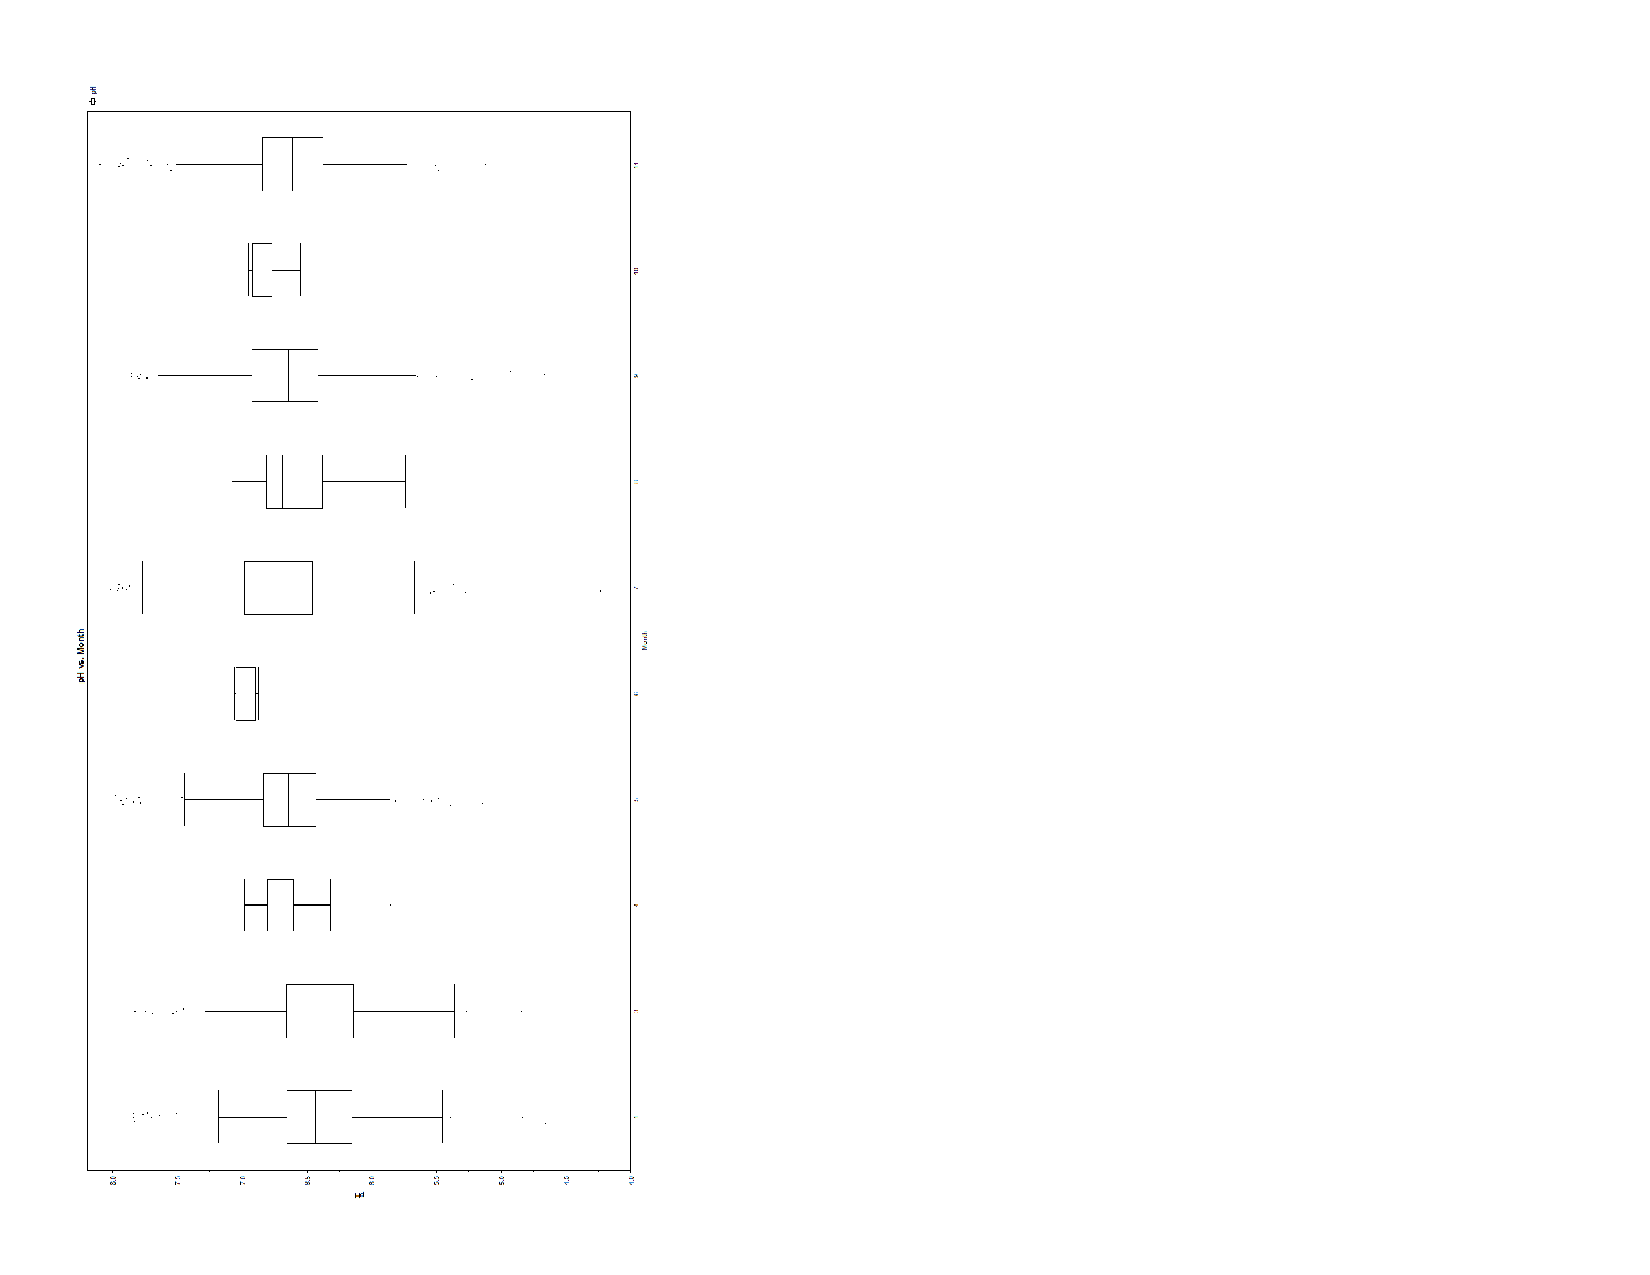
\includepdf[noautoscale,scale=1.45,offset=350 0,pages=-,linktodoc]{figures/CAGraph1}

\phantomsection
\label{CAGraph2}
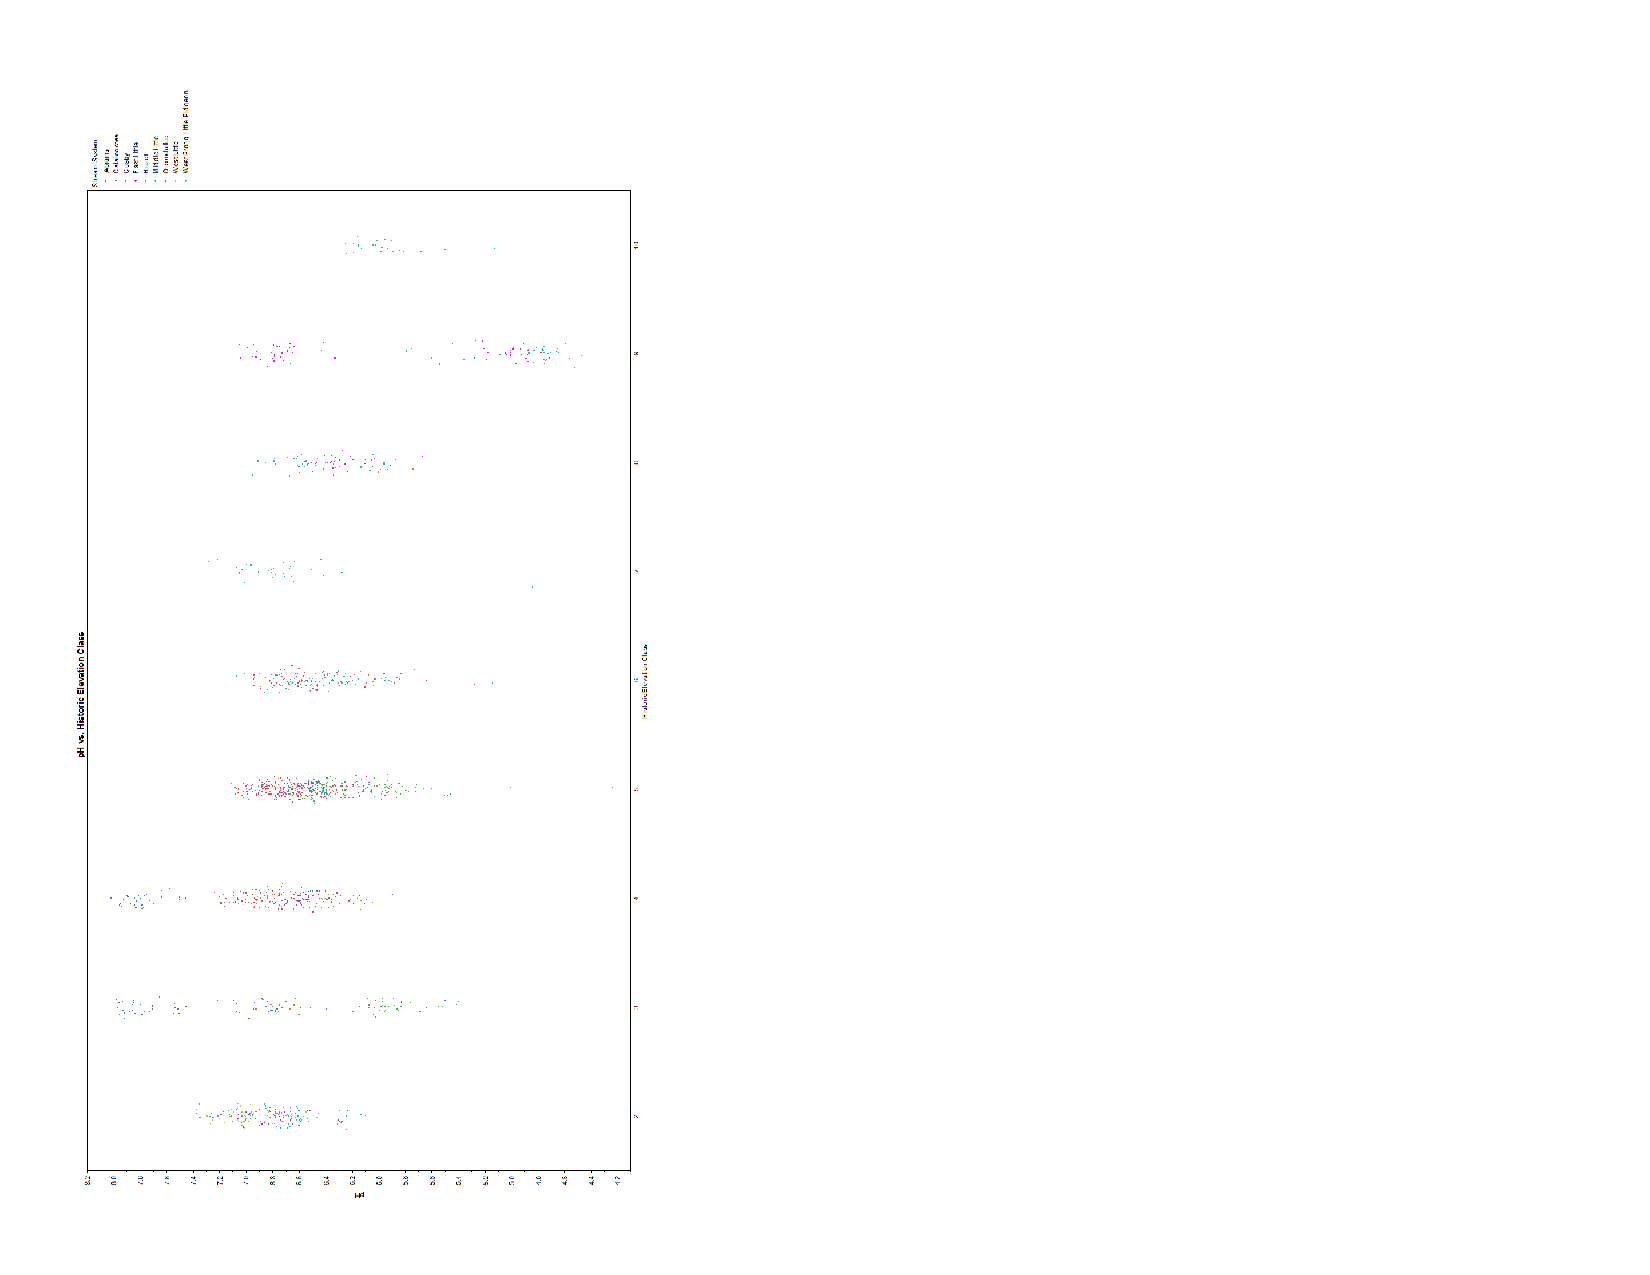
\includepdf[noautoscale,scale=1.45,offset=350 0,pages=-,linktodoc]{figures/CAGraph2}

\phantomsection
\label{CAGraph3}
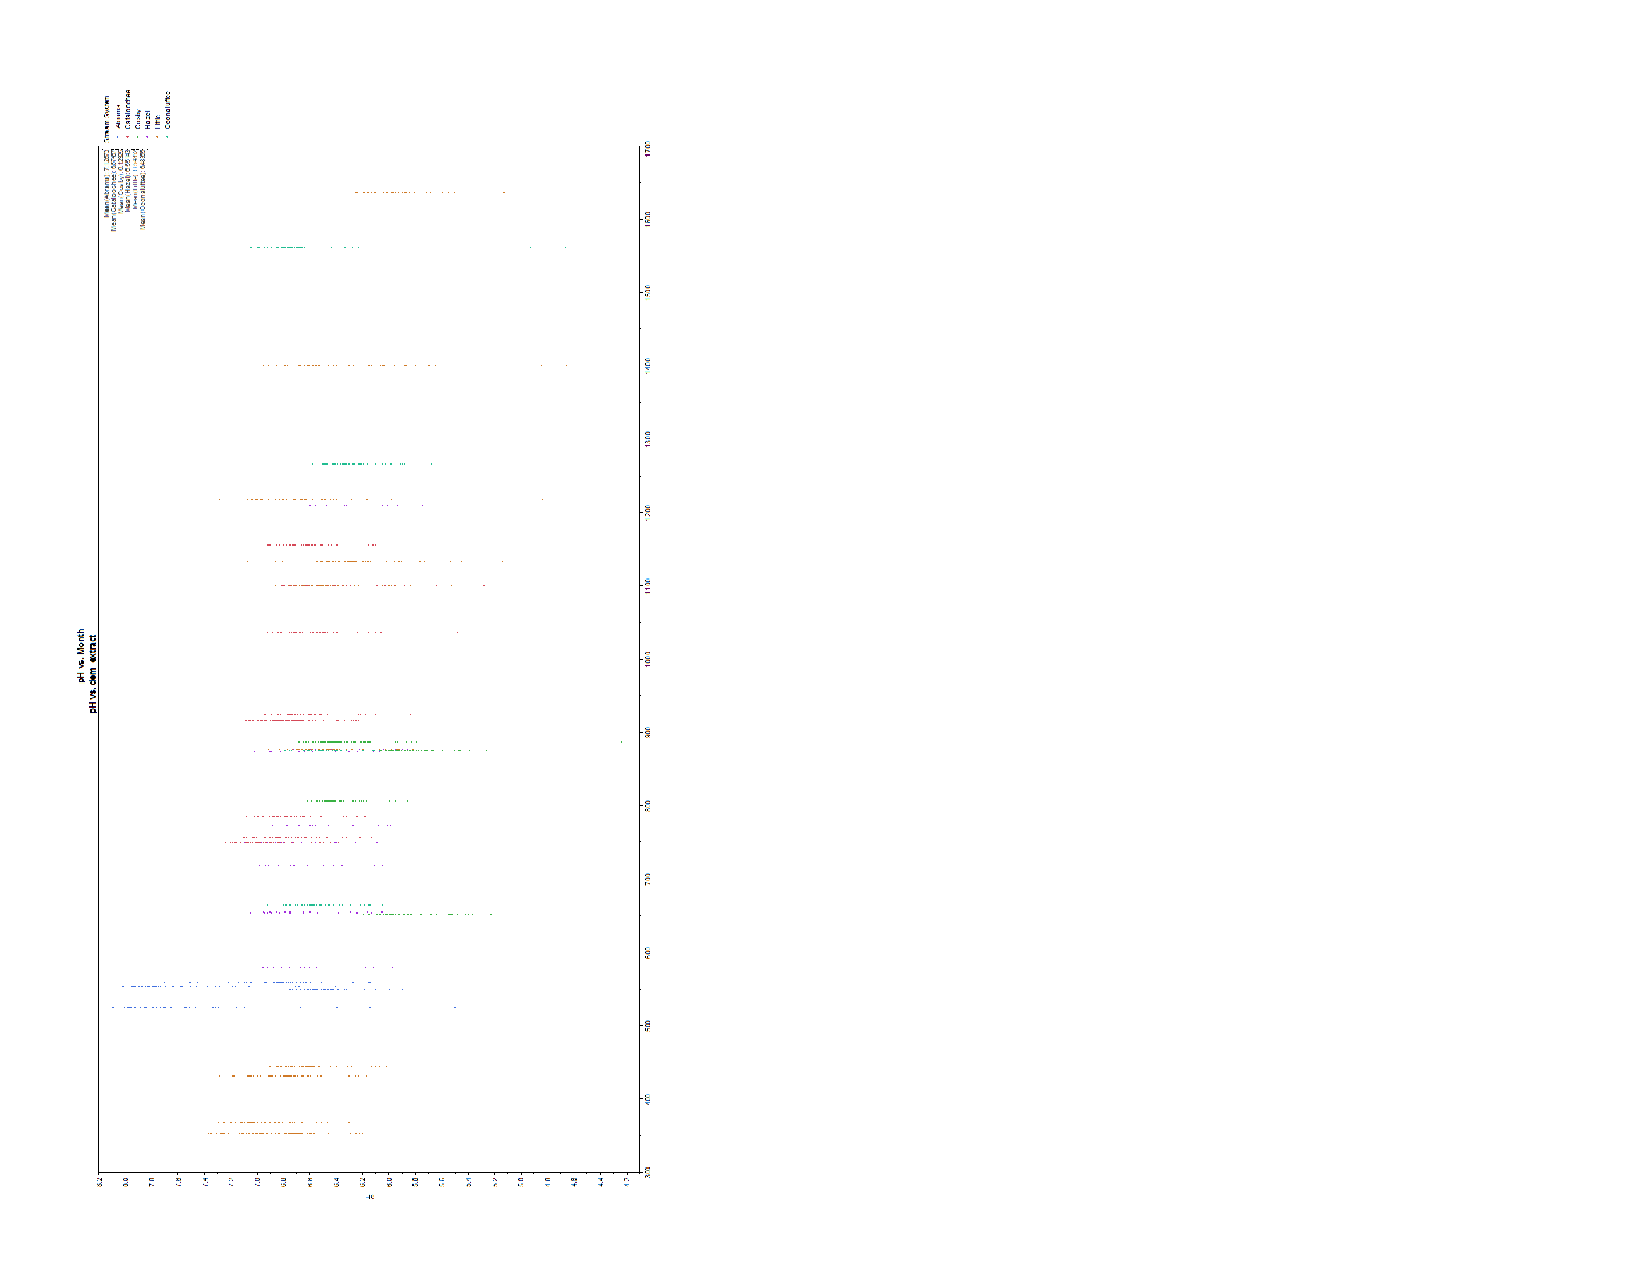
\includepdf[noautoscale,scale=1.45,offset=350 0,pages=-,linktodoc]{figures/CAGraph3}

\phantomsection
\label{CAGraph6}
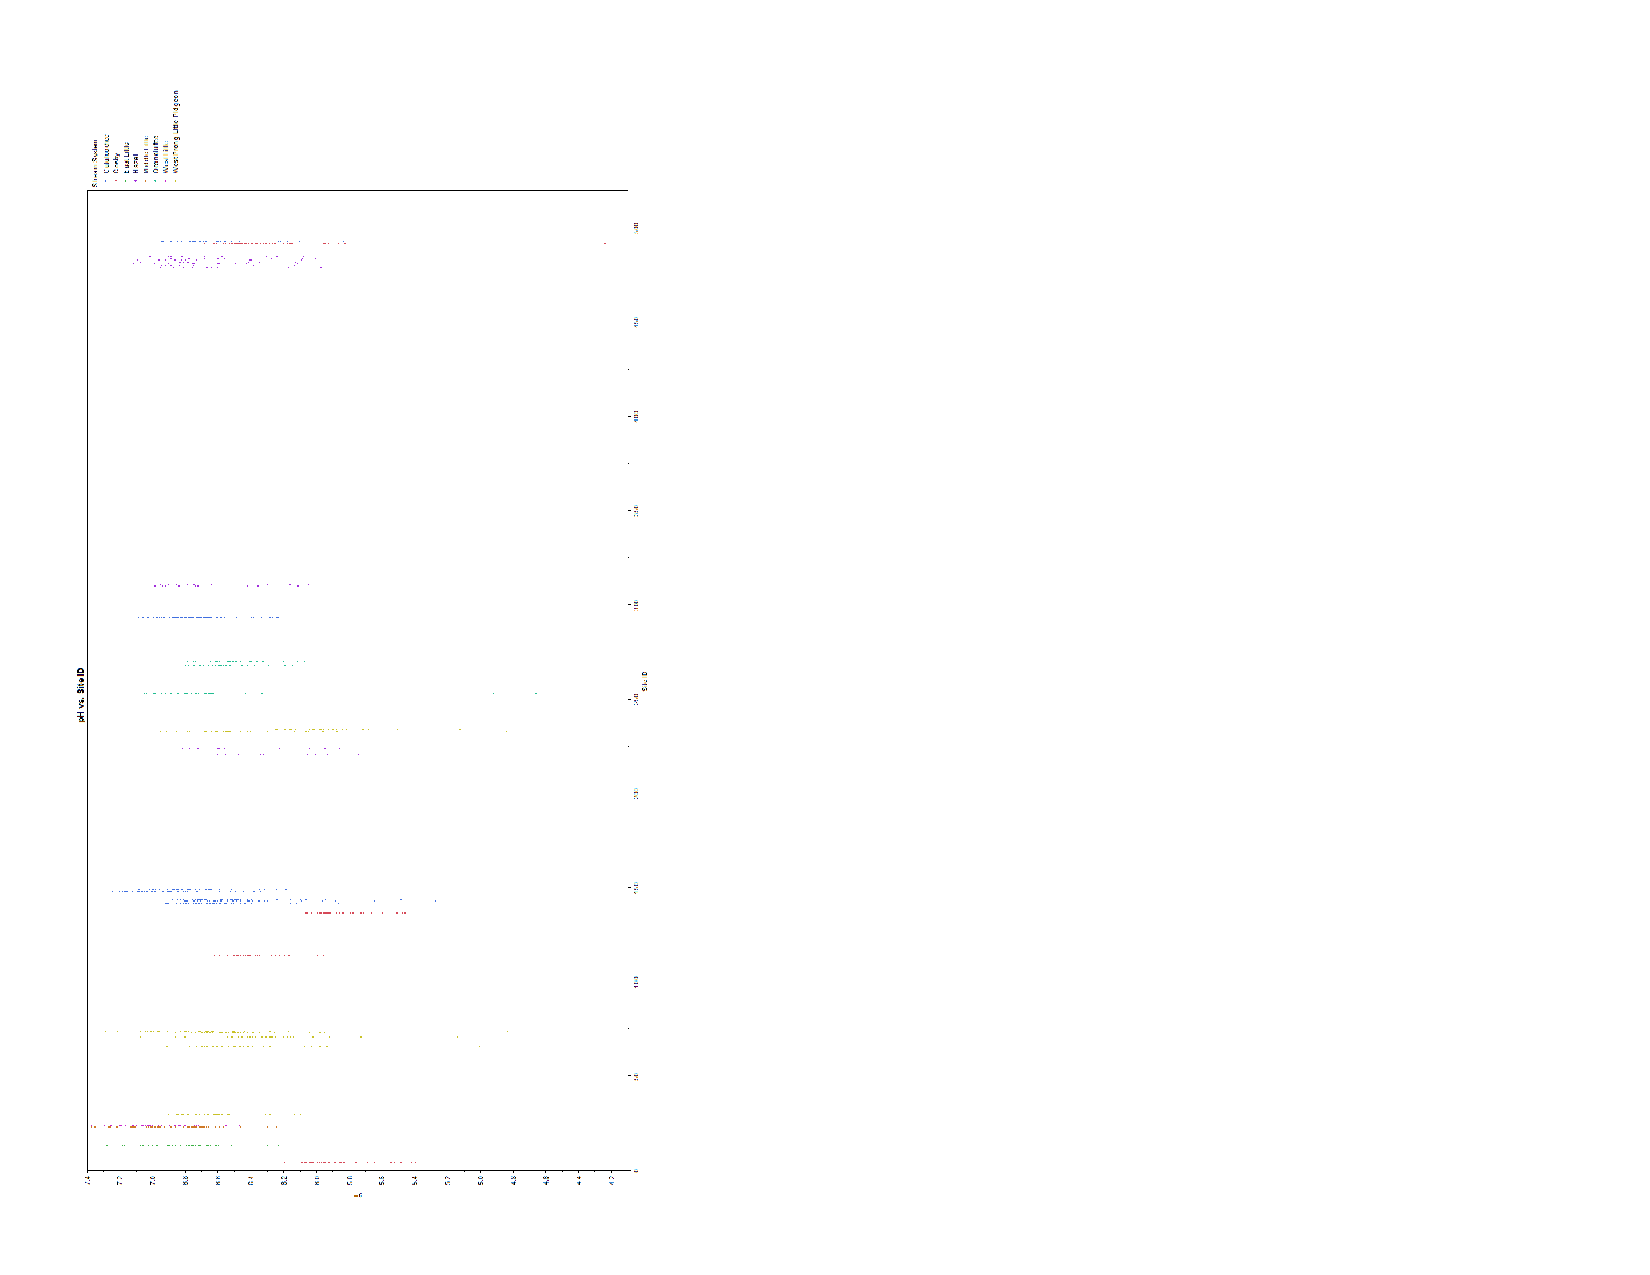
\includepdf[noautoscale,scale=1.45,offset=350 0,pages=-,linktodoc]{figures/CAGraph6}

\phantomsection
\label{CAGraph8}
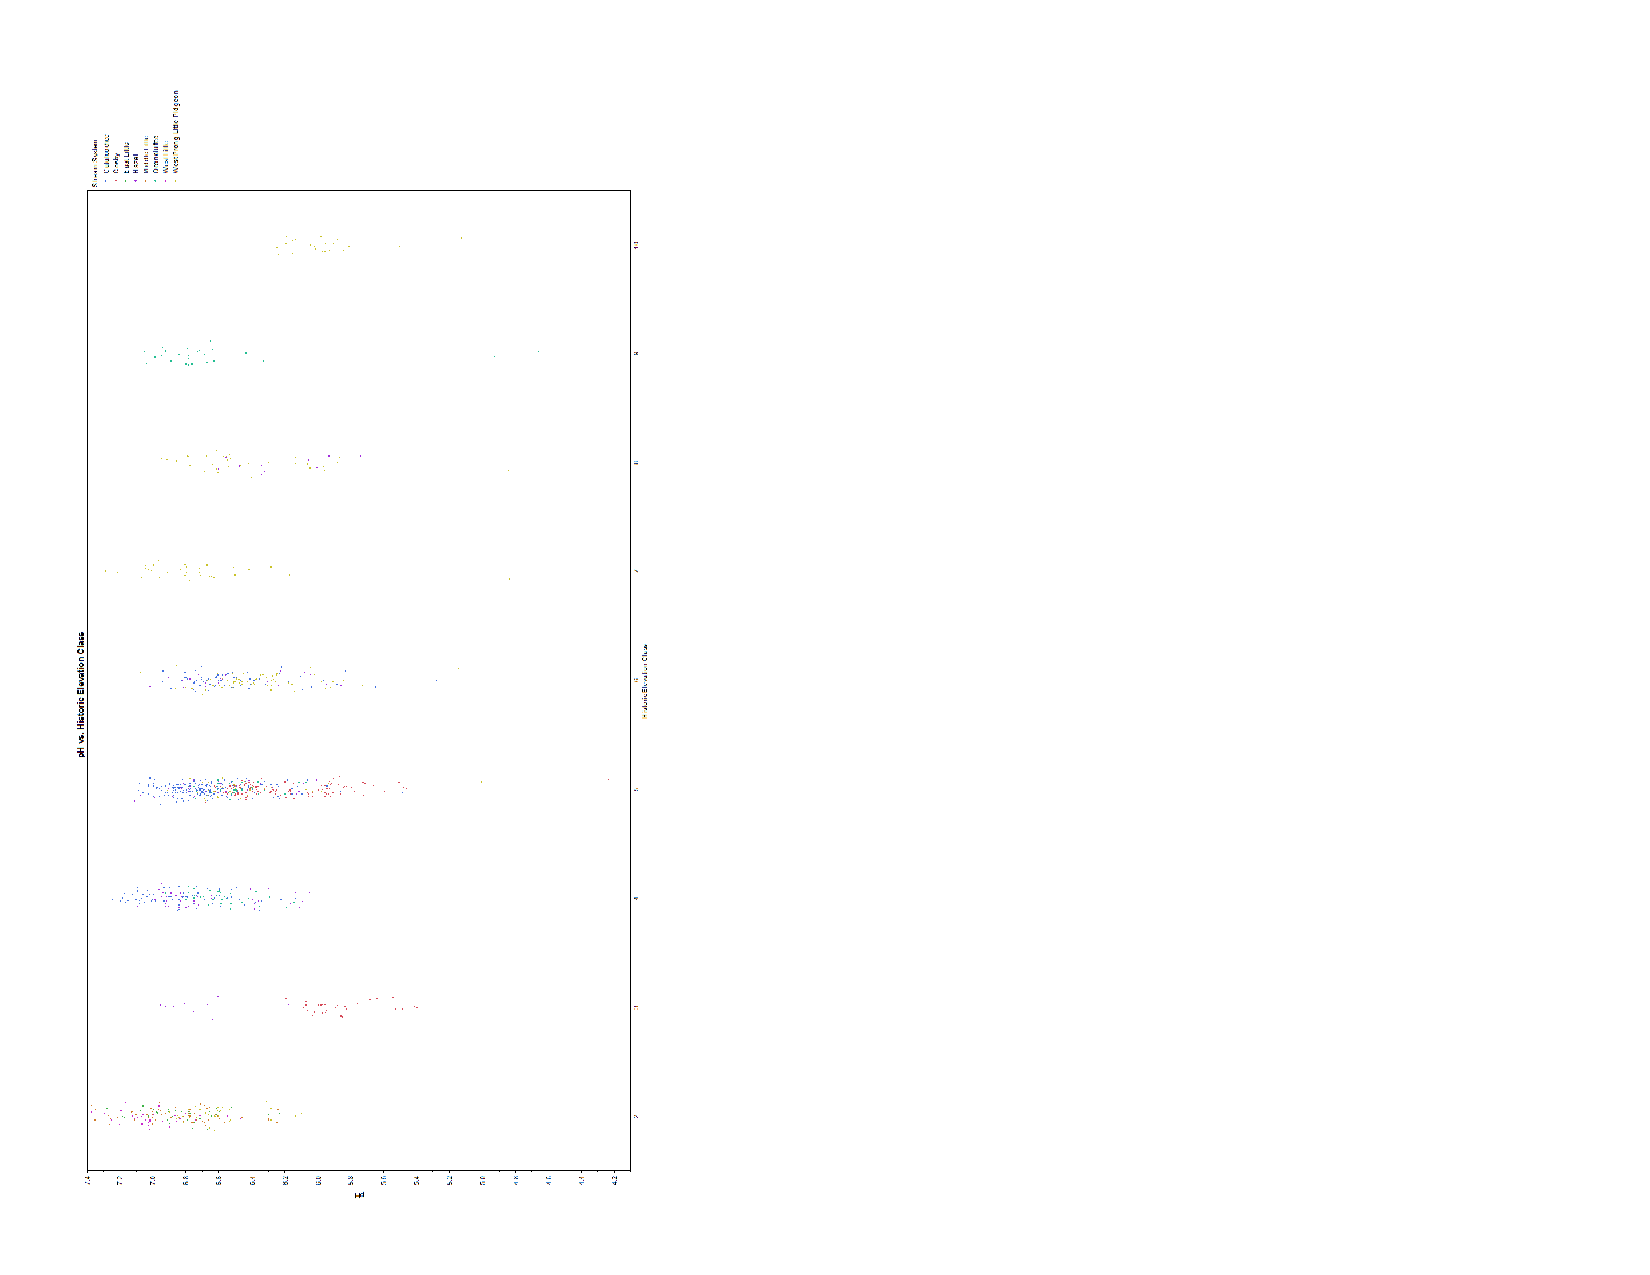
\includepdf[noautoscale,scale=1.45,offset=350 0,pages=-,linktodoc]{figures/CAGraph8}

\phantomsection
\label{CAGraph9}
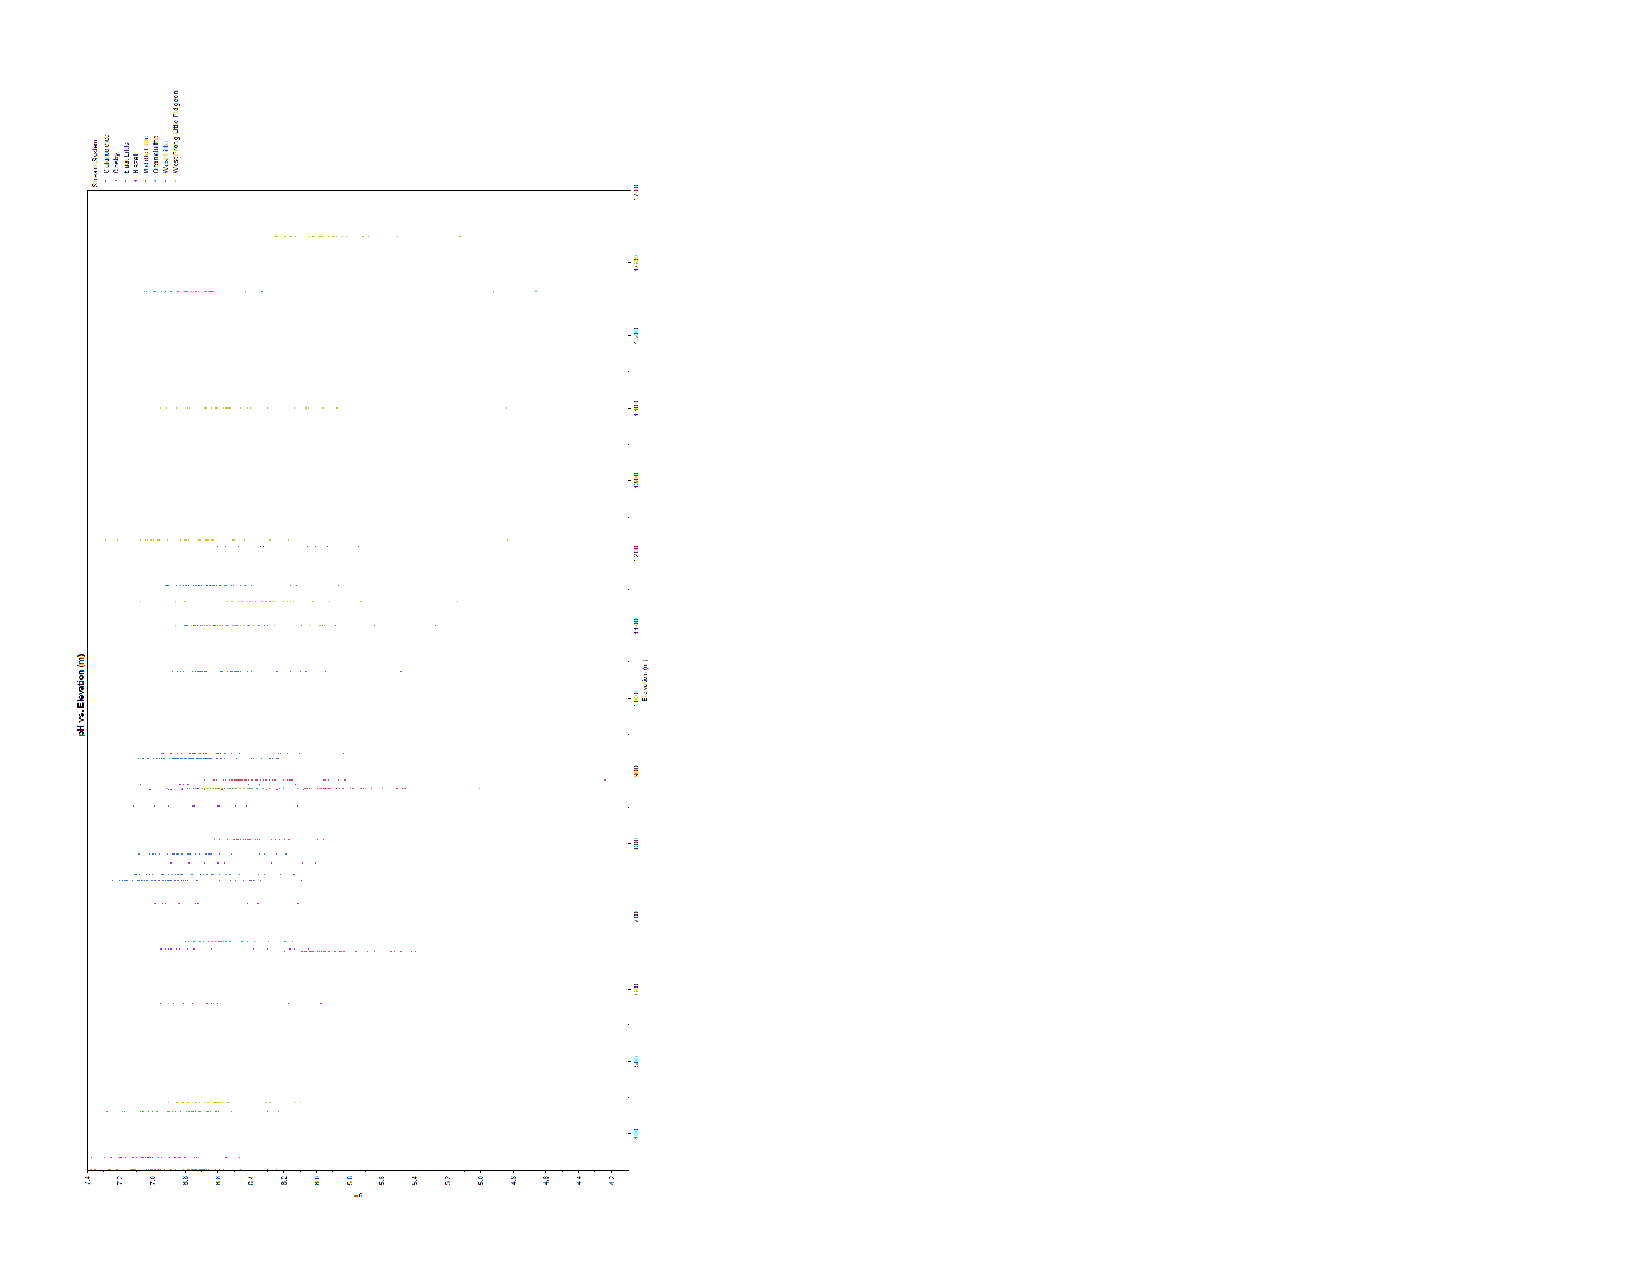
\includepdf[noautoscale,scale=1.45,offset=350 0,pages=-,linktodoc]{figures/CAGraph9}

\phantomsection
\label{CAGraph10}
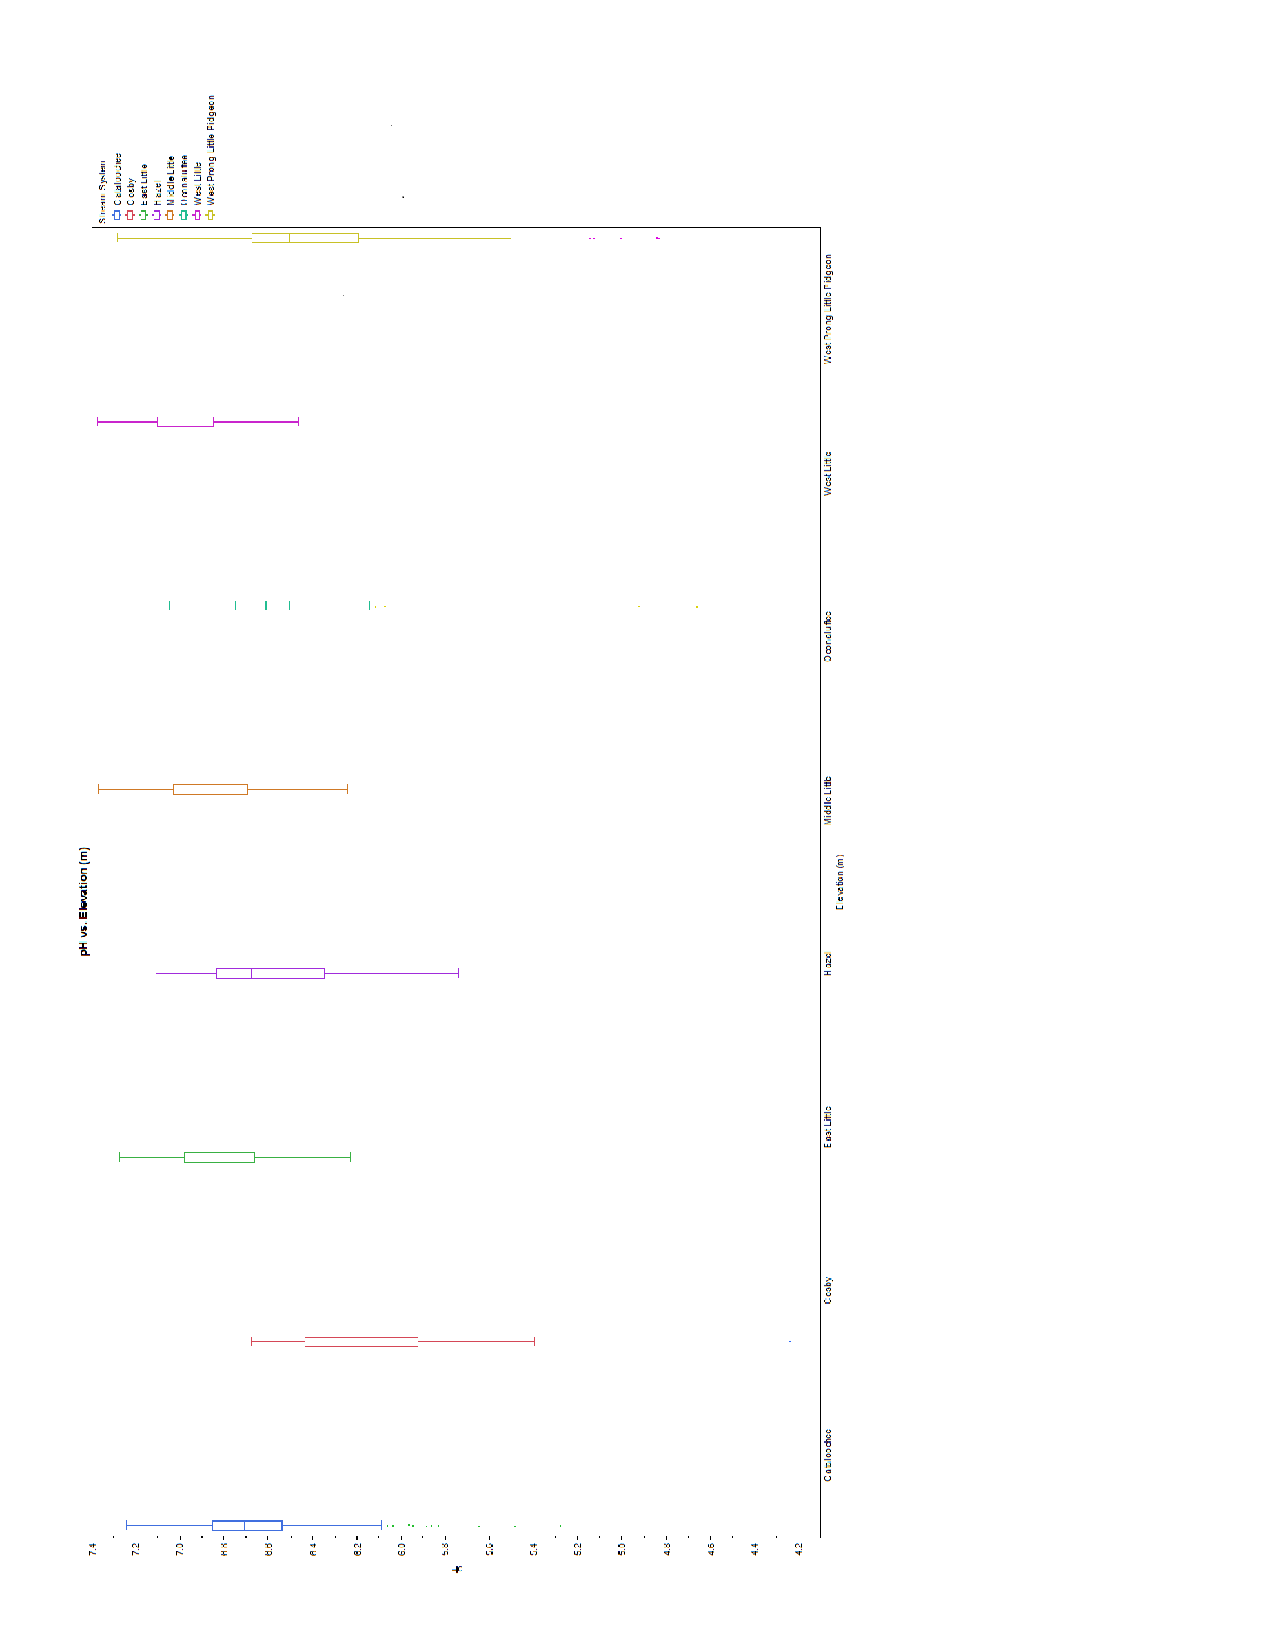
\includepdf[noautoscale,scale=1,offset=100 0,pages=-,linktodoc]{figures/CAGraph10}


\end{document}
